% ==============================================================================
% RESULTADOS
% ==============================================================================
% Instrucciones de la plantilla:
% - Por cada una de las actividades, describir detalladamente los resultados
%   alcanzados, tanto de las solicitadas, como de los experimentos.
% - Incluir capturas de pantalla debidamente tituladas y referenciadas en el texto.
% - REGLA: No se aceptarán solo capturas de pantalla; deben estar explicadas.
% - Analizar ventajas y desventajas de la metodología aplicada.
% ==============================================================================

\section{Resultados}

A continuación se presentan los resultados de cada actividad. Todas las capturas de OpenGL corresponden al programa compilado en Visual Studio con la configuración \texttt{Debug|x64}.

% ------------------------------------------------------------------------------
\subsection{Resultados del Objeto 1: casa con el modelo de Phong}
La Figura \ref{fig:objeto1_final} muestra la casa con todas las modificaciones de los experimentos: el \textit{shader} con las tres componentes de Phong multiplicadas por la textura (Listado \ref{lst:phong_fs}) y los parámetros finales del Listado \ref{lst:parametros}, es decir, luz blanca de potencia 60 en $(0, 5, 0)$, exponente especular de 10, material con ambiental gris de 0.3, difusa rojiza, especular azul y transparencia de 0.5. La música se reproduce en bucle desde que se abre la ventana.

\begin{figure}[H]
    \centering
    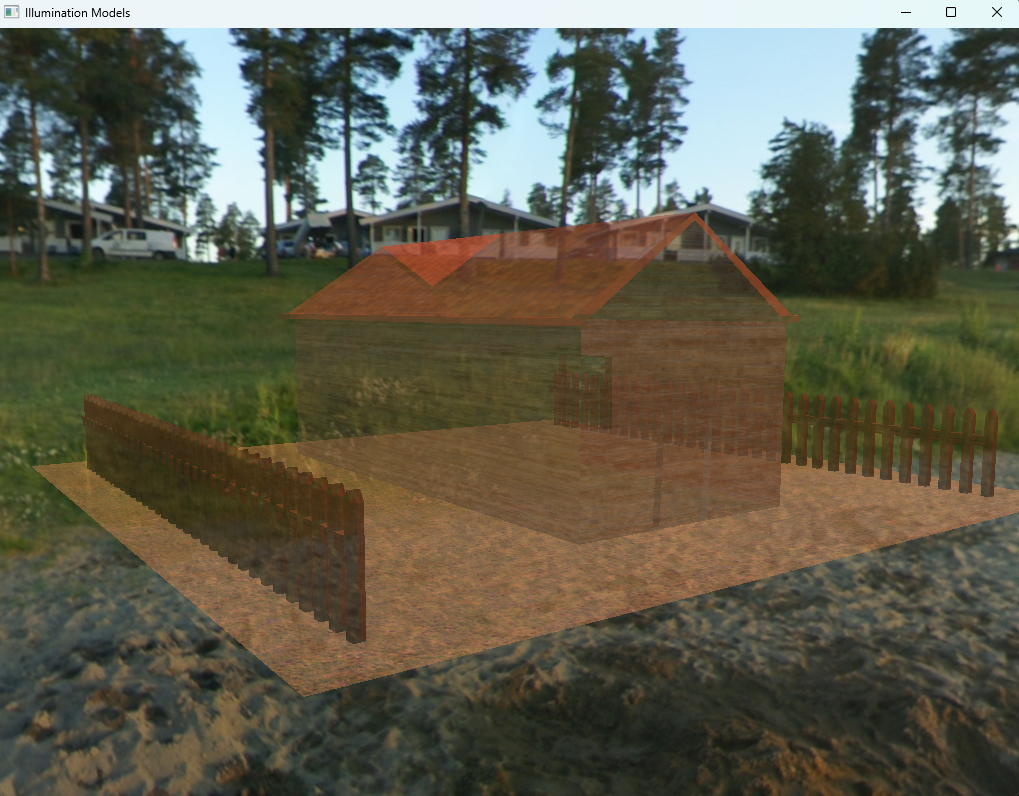
\includegraphics[width=0.75\textwidth]{Imagenes/Objeto1/objeto1ef.png}
    \caption{Resultado final del Objeto 1: casa semitransparente iluminada con el modelo de Phong y texturizada.}
    \label{fig:objeto1_final}
\end{figure}

La transparencia se aplica a todo el modelo, porque el material es uno solo para todas las mallas del FBX. A través de las paredes se ven la cerca del fondo, el interior de la casa y los árboles del cubemap, y la madera y la teja conservan su textura. La componente ambiental aporta $0.3 \times 2.4 = 0.72$ en cada canal, suficiente para que las caras que no reciben luz directa se vean sin quedar negras. Sobre ella, la componente difusa roja da el tono anaranjado del terreno y del techo, las superficies que miran hacia la luz. Con el exponente de 10 el brillo especular azul queda reducido a zonas pequeñas, y ya no tiñe caras completas como en el Experimento 4.

En el techo se nota una zona en forma de V con una opacidad distinta a la del resto. La mezcla de colores depende del orden en que se dibujan las caras, y el programa dibuja el modelo con la prueba de profundidad activa y sin ordenar los triángulos de atrás hacia adelante. Cuando una cara cercana se dibuja antes que otra que está detrás, escribe su profundidad y la de atrás se descarta, así que en esa zona la cara lejana no se mezcla.

\subsubsection{Análisis de ventajas y desventajas}
\begin{itemize}
    \item \textbf{Ventajas:} El modelo de Phong se calcula por fragmento con unas cuantas operaciones vectoriales, y separar las tres componentes permite ajustar cada una con un solo parámetro del \texttt{main} sin tocar el \textit{shader}. Multiplicar la iluminación por la textura conserva el detalle del modelo, y la transparencia solo necesitó un \textit{uniform} y la mezcla de OpenGL.
    \item \textbf{Desventajas:} La atenuación usa una distancia fija, de modo que la luz no se debilita al alejarla. Con la potencia de 60 los coeficientes del material se saturan con facilidad (cualquier ambiental mayor que 0.42 deja la casa blanca). Además, \texttt{alphaIndex} es entero y no admite exponentes menores que 1, y la transparencia muestra errores de orden de dibujo porque las caras no se ordenan por profundidad.
\end{itemize}

% ------------------------------------------------------------------------------
\subsection{Resultados del Objeto 2: planeta de la práctica 6}
La Figura \ref{fig:objeto2_final} muestra el planeta con los parámetros finales del Listado \ref{lst:parametros_objeto2}: luz blanca de potencia 60 en $(4, 2, 3)$, exponente especular de 30 y material gris con ambiental de 0.05, difusa de 0.4 y especular de 0.3, sin transparencia. La música es la misma del Objeto 1.

\begin{figure}[H]
    \centering
    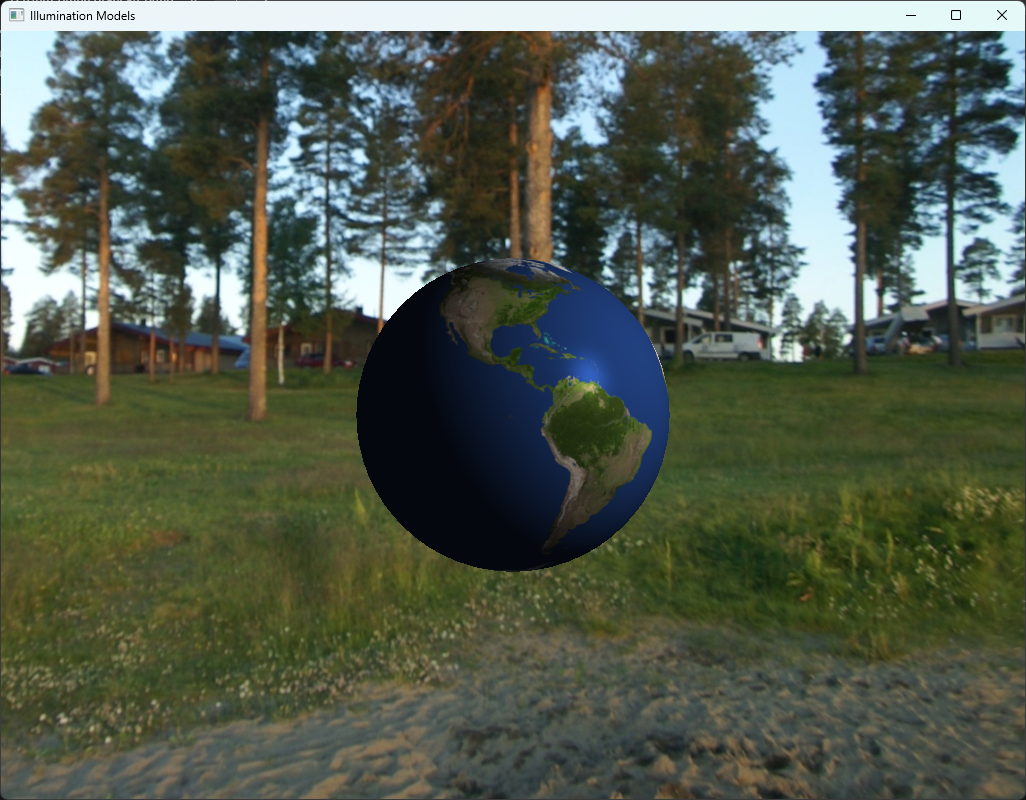
\includegraphics[width=0.75\textwidth]{Imagenes/Objeto2/objeto2ef.png}
    \caption{Resultado final del Objeto 2: el planeta iluminado como la Tierra por el Sol, con el lado de día, el de noche y el reflejo sobre el Caribe.}
    \label{fig:objeto2_final}
\end{figure}

Cada componente de Phong se distingue en la imagen. La difusa ilumina la mitad derecha del planeta y se oscurece de forma gradual hacia la izquierda conforme crece el ángulo entre la normal y la dirección de la luz. Al pasar los 90°, el \texttt{clamp} la deja en cero y solo queda la ambiental, que hace visible el lado de noche apenas como un azul muy oscuro. La especular forma un brillo pequeño sobre el mar, entre Centroamérica y el Caribe, en la zona donde el reflejo de la luz apunta hacia la cámara. Como el material es gris, los continentes y el mar conservan los colores de la textura de la práctica 6.

Comparado con el Objeto 1, el planeta muestra mejor el modelo porque su normal cambia de forma continua: el degradado de la componente difusa y el lóbulo de la especular se ven completos en una sola imagen, mientras que en la casa cada pared tiene un solo tono. Además, como el planeta es opaco, no aparecen los errores de orden de dibujo del Experimento 7.

\subsubsection{Análisis de ventajas y desventajas}
\begin{itemize}
    \item \textbf{Ventajas:} Reutilizar el modelo de la práctica 6 solo requirió exportarlo de nuevo con un script y cambiar seis líneas del programa, sin tocar el \textit{shader}, y se conservó la numeración del archivo. Con un material gris, la iluminación de Phong se suma a la textura sin cambiar sus colores.
    \item \textbf{Desventajas:} El reflejo especular se multiplica por la textura y sobre el mar se ve azul en lugar de blanco; habría que sumar la componente especular después de aplicar la textura. La frontera entre el día y la noche es más brusca que en la Tierra real, porque el modelo no simula la atmósfera. La luz tampoco se debilita con la distancia, porque la atenuación usa el valor fijo de \texttt{distance}.
\end{itemize}
